\documentclass[letterpaper,11pt]{article}
\usepackage{graphicx}
\usepackage{listings}
\usepackage[super]{nth}
\usepackage[hyphens]{url}
\usepackage{hyperref}
\usepackage{amsmath}
\usepackage[makeroom]{cancel}
\usepackage[table]{xcolor}
\usepackage{comment}
\usepackage[space]{grffile}
\usepackage{csvsimple}
\usepackage{longtable}
\usepackage{adjustbox}


\newcommand*{\srcPath}{../src}%

\lstset{
	basicstyle=\footnotesize,
	breaklines=true,
}

\begin{document}

\begin{titlepage}

\begin{center}

\Huge{Assignment 1}

\Large{CS 734:  Introduction to Information Retrieval}

\Large{Fall 2017}

\Large{Grant Atkins}

\Large Finished on \today

\end{center}

\end{titlepage}

\newpage


% =================================
% First question
% =================================
\section*{1}

\subsection*{Question}

\begin{verbatim}
1.2 	Site Search is another common application of search engines. 
In this case, search is restricted to the web pages at a given website. 
Compare site search to web search, vertical search, and enterprise search.
\end{verbatim}

\subsection*{Answer}

To answer this question I decided to use the search query ``cs834-f17'' with modifications as necessary across each of these search types. 
For site search I used github.com as our course repository is hosted on github and will likely return results and as the name site search implies it only searches on the designated website.
Google offers the option to site search with the command ``site:website'' which for my entry it is ``cs834-f17 site:github.com''  as shown in Figure \ref{fig:sitesearch} \cite{googlesite}.
It only returned two results which is minimal and as expected because it is a unique term and the term ``cs834-f17'' isn't expected to be located in any other repository or description hosted on github.

For web search I continued to use google. Using the query term ``cs834-f17'' this time without specifying anything else returned 57 results as shown in Figure \ref{fig:websearch}. 
Both web search and site search both return the same top result, which is the repository. Something that is interesting in this search is that it didn't show the second result
from the site search. Instead the web search went to different domains to try and find ``cs834-f17'', for example \textit{github.io}. This should be noted as the precision in site search
is seems to be more effective in the context of terms. 

Continuing with vertical search I also made use of google images. The goal of vertical search is to search on a specific content type.
The results were somewhat expected as there was in fact a picture of the author of the cs834-f17 repository, Dr. Nelson as shown in Figure \ref{fig:verticalsearch}, however prior to that image it seems of had lot of patent schemes for protein formulas. In this context it probably wasn't the best to use a vertical search.

Finally when completing Enterprise search it should be noted that I don't have access to an intranet but I do have access to my own personal machine to conduct searches on my own file system. 
I used my operating system's implemented search in it file system and I also use the terminal command \textit{grep} to show a customized search on a subset of directories.
Using my operating systems \textit{finder} program it searches across my entire computer of files with the words ``cs834-f17'' as shown in Figure \ref{fig:esearch1}. This type of seems more relatable to web search as it seem to generalize the results showing files that mention this term, but not every single file in my filesystem.
When I used the \textit{grep} command searching any directories starting with ``cs'' it showed every occurrence where ``cs834-f17'' was used. This is more relatable to site search because it listed all locations of occurrence in these directories.

  \begin{figure}[h]
  \centering
  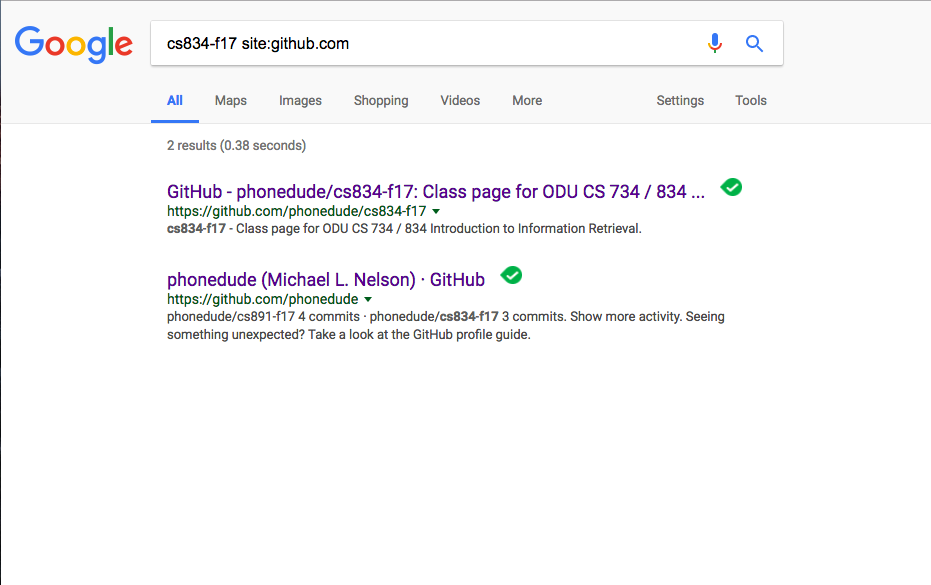
\includegraphics[scale=0.4]{sitesearch.png}
  \caption{Site search example in google}
  \label{fig:sitesearch}
  \end{figure}

  \begin{figure}[h]
  \centering
  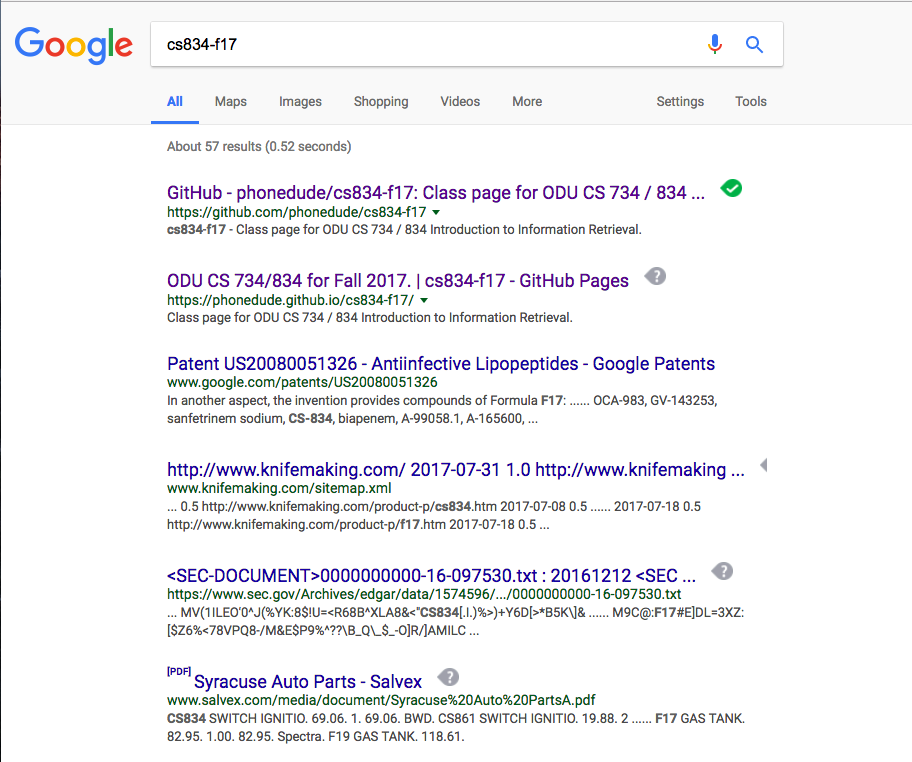
\includegraphics[scale=0.4]{websearch.png}
  \caption{Web search example in google}
  \label{fig:websearch}
  \end{figure}
  
   \begin{figure}[h]
  \centering
  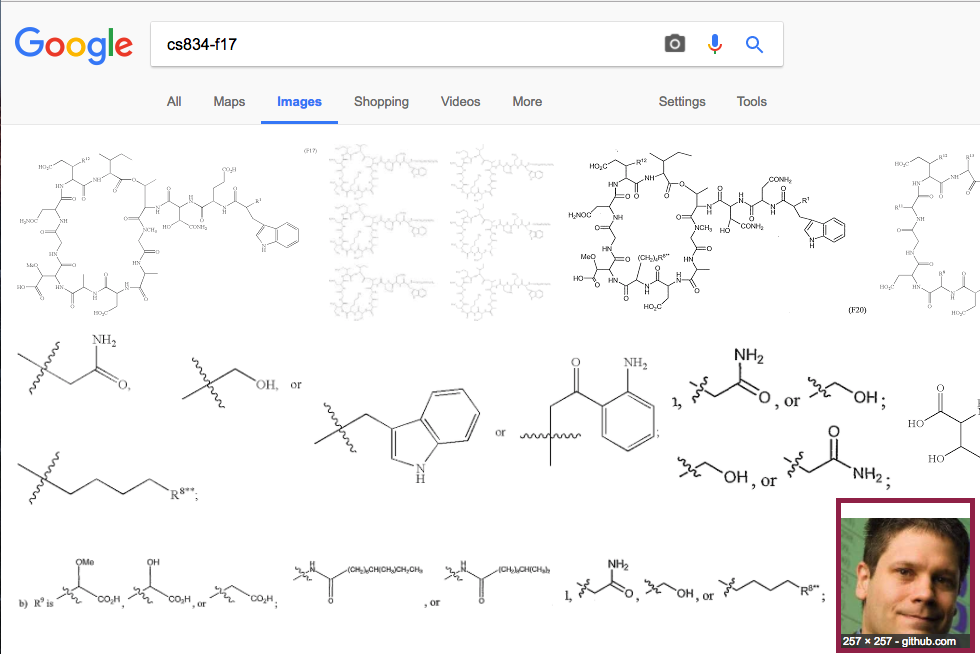
\includegraphics[scale=0.4]{verticalsearch.png}
  \caption{Vertical search example in google}
  \label{fig:verticalsearch}
  \end{figure}
  
   \clearpage
  \begin{figure}[h]
  \centering
  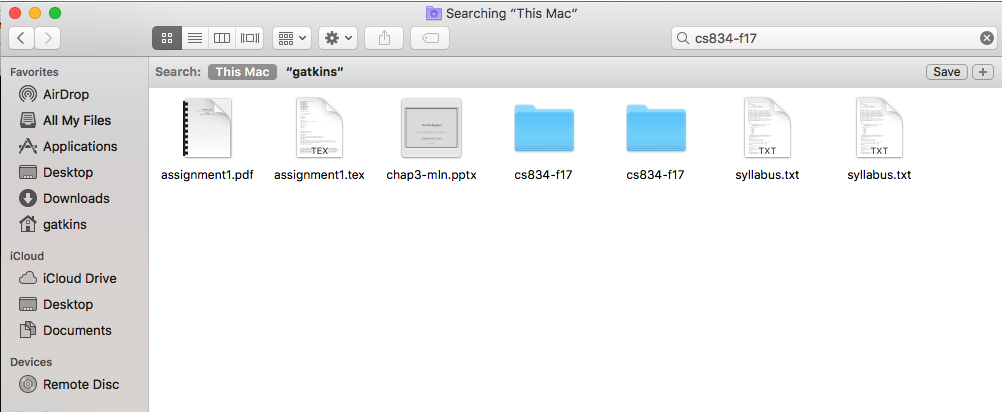
\includegraphics[scale=0.4]{filesystemsearch.png}
  \caption{Enterprise Search using my own Desktop}
  \label{fig:esearch1}
  \end{figure}

  \begin{figure}[h]
  \centering
  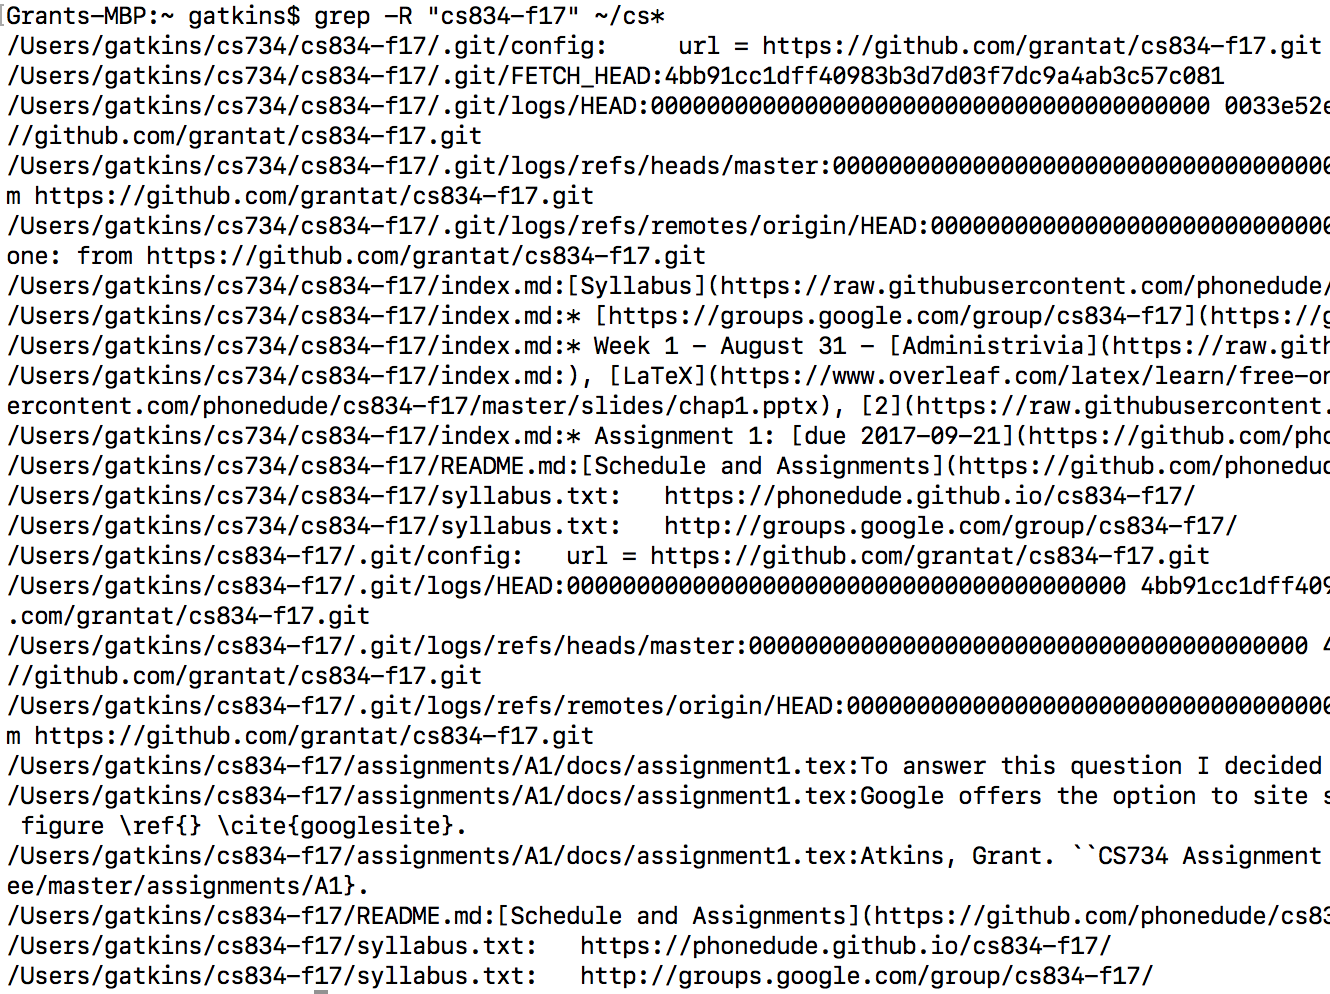
\includegraphics[scale=0.35]{grepsearch.png}
  \caption{Specified Enterprise Search using my own Desktop in a terminal}
  \label{fig:esearch2}
  \end{figure}


\clearpage

% =================================
% Second question
% =================================

\section*{2}

\subsection*{Question}

\begin{verbatim}
1.4 	List five web services or sites that you use that appear to use search, 
not including web search engines. Describe the role of search for that 
service. Also describe the search is based on a database or grep style
of matching, or if the search is using some type of ranking.
\end{verbatim}

\subsection*{Answer}

Five websites with web services I use frequently that use some sort of search mechanism include: \url{quora.com}, \url{github.com}, \url{twitter.com}, \url{youtube.com}, and quite recently \url{docs.docker.com}.

Quora is a popular question answer website based on topics. This website include a mixed search type of database querying and grep style. As shown below in Figure \ref{fig:quora}, if I start to search for ``webscience'' it will start to autocomplete it showing topics where that entry contains grep but not an exact match of the term. It also uses databases for storing these topics and a full text search of a topic is allowed which return all entries of that topic.

\begin{figure}[h]
\centering

\includegraphics[scale=0.35]{quora.png}
\caption{Quora search example}
\label{fig:quora}
\end{figure}

Github also includes a database and grep style of searching. When I search for ``swift'' on github it shows the following containing this term: repositories, code, commits, issues, wikis, and users as shown in Figure \ref{fig:github}. This is obviously a grep for in-text occasions. However, the URI gives away a hint of database querying for a REST interface for example the following URI was sent for this term search: \url{https://github.com/search?utf8=%E2%9C%93&q=swift&type=}

\begin{figure}[h]
\centering
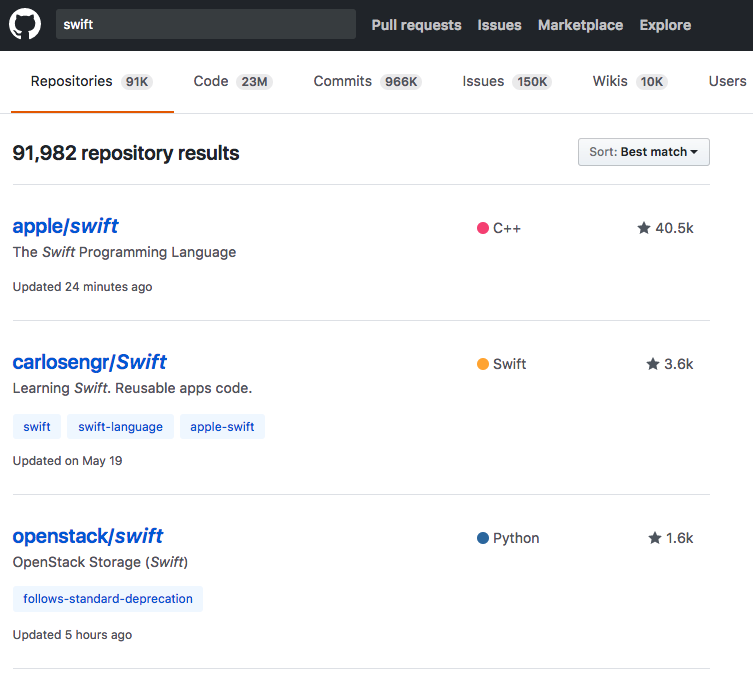
\includegraphics[scale=0.35]{github.png}
\caption{Github search example}
\label{fig:github}
\end{figure}

Twitter is based on database searching. It uses services to take the input of a user then queries in their database.
This request is then filtered down to 10 items whether it be users, hashtags, or topics as shown in Figure \ref{fig:twitter}.
Each of these items is tagged which is noted in their database for tracking.

\begin{figure}[h]
\centering

\includegraphics[scale=0.35]{twitter.png}
\caption{Twitter search example}
\label{fig:twitter}
\end{figure}

Youtube is my go to for music and any other video content. 
Youtube uses a database for its search with an example query shown in Figure \ref{fig:youtube}. 
When you track a request from youtube you'll see an outgoing request be sent to their services. 
When the request is done you'll see the videos starting with your query term but when you follow that link it is based on a hash which is stored somewhere in database.

\begin{figure}[h]
\centering
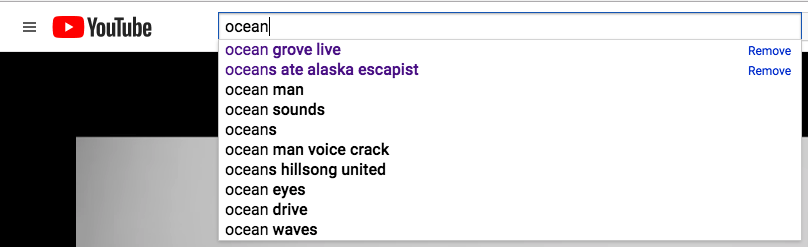
\includegraphics[scale=0.35]{youtube.png}
\caption{Youtube search example}
\label{fig:youtube}
\end{figure}

The docker docs, \url{docs.docker.com} is something I've been using quite frequently lately and I've noticed that this search is strictly a grep search. 
Document websites for software are more often than not, built statically meaning they produce these files separately for each location on the website as shown in Figure \ref{fig:docker}.
Also a sure tell for this is usually done by looking at network activity and for this website it showed no outgoing request on a search.

\begin{figure}[h]
\centering
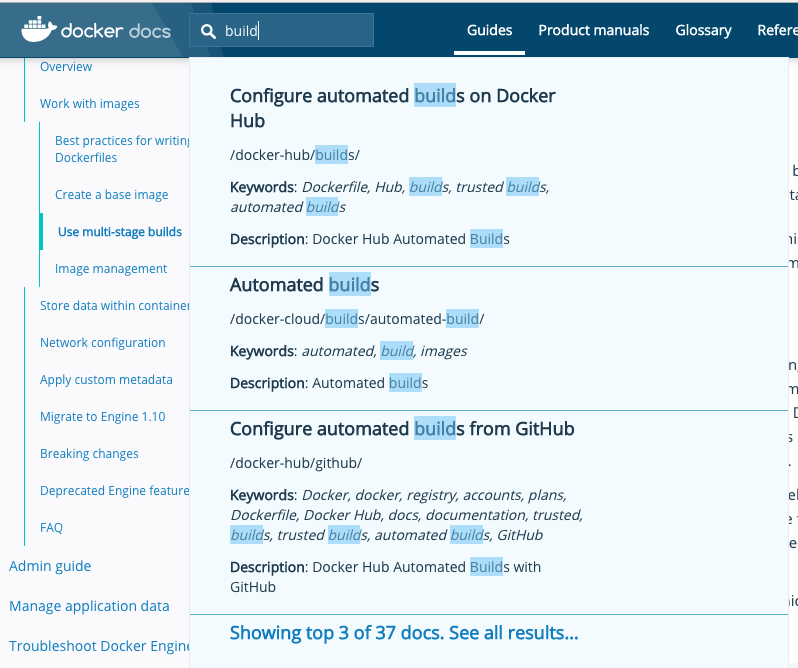
\includegraphics[scale=0.35]{docker.png}
\caption{Docker docs search example}
\label{fig:docker}
\end{figure}


\clearpage

% =================================
% 3rd question
% =================================

\section*{3}

\subsection*{Question}

\begin{verbatim}
3.7 	Write a program that can create a valid sitemap based on the 
contents of a directory on your computer's hard disk. Assume 
the file are accessible from a website at the URL http://example.com. 
For instance, if there is a file in your directory called homework.pdf, 
this would be available at http://www.example.com/homework.pdf. 
Use the real modification date on the file as the last modified time in the 
sitemap, and to help estimate the change frequency.
\end{verbatim}

\subsection*{Answer}

To answer this question a wrote a program in Python 3.0+ as shown in Listing \ref{lst:sitemap}. 
This program selects a directory from which to build a sitemap.
The directory I decided to use for this question was actually this assignment's directory, \textbf{A1}, for this course's repository \cite{github}.
The XML sitemap genered is shown in Listing \ref{lst:sitemap_output}. 
It should be noted that you won't see a \textbf{.DS\_Store} or some of the other LaTeX files located in the \textbf{/A1/docs/} folder in this 
repository due to them being ignored in my repository's \textbf{.gitignore} file, these files are in fact on my computer locally. 


 \lstinputlisting[frame=single,caption={Python script create a sitemap from a directory's contents},label=lst:sitemap,captionpos=b,numbers=left,showspaces=false,showstringspaces=false,basicstyle=\footnotesize]{\srcPath/sitemap.py}

 \lstinputlisting[frame=single,caption={Sitemap created from my assignment 1 (A1) directory},label=lst:sitemap_output,captionpos=b,numbers=left,showspaces=false,showstringspaces=false,basicstyle=\footnotesize]{\srcPath/data/sitemap.xml}

\clearpage

% =================================
% 4th question
% =================================

\section*{4}

\subsection*{Question}

\begin{verbatim}
Suppose that, in an effort to crawl web pages faster, you set up two crawling 
machines with different starting seed URIs. Is this an effective strategy for 
distributed crawling? Why or why not.
\end{verbatim}

\subsection*{Answer}

This is not an effective strategy for distributed crawling. 
An important idea to remember is that the web is a graph structure where many links will eventually connect to one another.
With this in mind, as these web crawlers start crawling through their assigned URIs and the depth in which the URIs in that page start to branch to other websites they will eventually overlap URIs which have either already been crawled or already in line to be crawled.
Recently for our paper presentations, I had to present a paper on IRLbot, a single server crawling bot which had answers to this sort of issue \cite{irlbot}.

With crawlers being separated by threads, IRLbot incorporated URI lookup and storage algorithms to track the URIs which I agree would be the best option. 
Whenever a URI is discovered it should be looked up inside the storage in which they track URIs and then cache the URI so the current crawlers can know even more quickly that they don't have to do a long search for this URI knowing its already been tracked.
If the system recognizes it as a new URI it will be able to add it to an active queue system to be crawled on. 
Again, since there are multiple crawlers the other crawlers can check the cache, the current URI queue, or a long lookup from storage if necessary.
Overall this system would prove faster than time lost performing requests to these servers and then checking if a URI can be stored.


\clearpage

% =================================
% 5th question
% =================================

\section*{5}

\subsection*{Question}

\begin{verbatim}
3.9 	Write a simple single-threaded web crawler. Starting from a single input 
URL (perhaps a professor's web page), the crawler should download a 
page and then wait at least five seconds before downloading the next 
page. Your program should find other pages to crawl by parsing link 
tags found in previously crawled documents.
\end{verbatim}

\subsection*{Answer}

This question was relatively simple as we were posed a question very similar to this question previously in our CS532 class except it had the goal of extracting all pdf files from a webpage and not chasing further links.
Therefore to answer this problem I used my code previously created from CS532 for assignment 1 but with some slight modifications as shown in Listing \ref{lst:crawler} \cite{cs532}.
For instance, I added: a time delay, a set to track the links already crawled, a queue system, and a hop counter for each website to track crawl level.
In this problem I tested 1 and 2 hops on the website \url{http://www.cs.odu.edu/~gatkins/cs725/}. 
With a max of 1 hop I found that I had queue size of 142 unique URIs remaining to crawl as shown in Figure \ref{fig:hop1}.
With a max of 2 hops I found that I had queue size of 2626 unique URIs remaining to crawl as shown in Figure \ref{fig:hop2}.

 \lstinputlisting[frame=single,caption={Python script to for a single-threaded web crawler},label=lst:crawler,captionpos=b,numbers=left,showspaces=false,showstringspaces=false,basicstyle=\footnotesize]{\srcPath/crawler.py}

\clearpage

\begin{figure}[h]
\centering
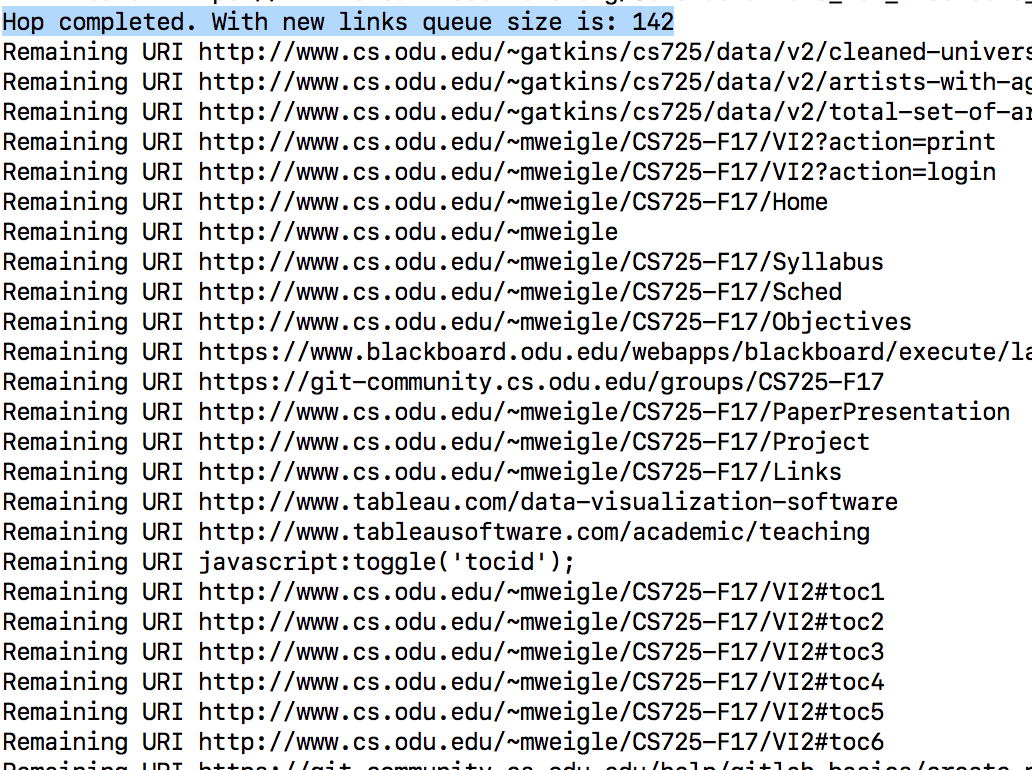
\includegraphics[scale=0.43]{hop1.png}
\caption{Terminal output of my crawler with 1 hop limit}
\label{fig:hop1}
\end{figure}

\begin{figure}[h]
\centering
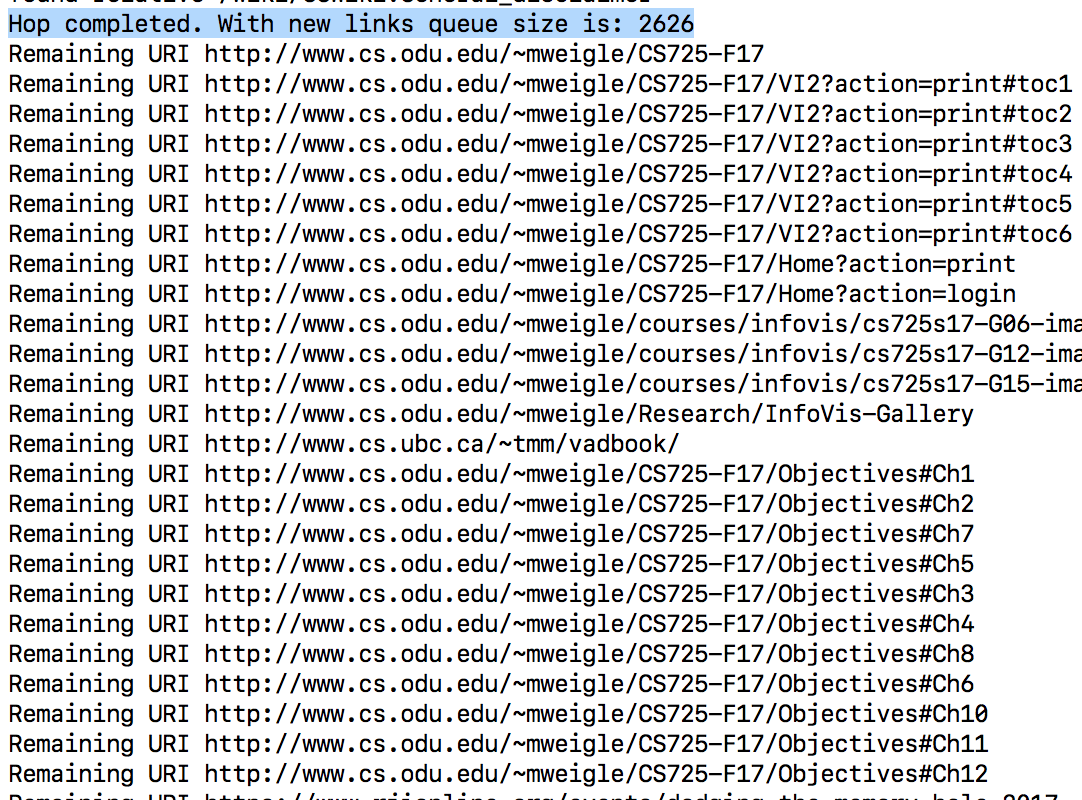
\includegraphics[scale=0.43]{hop2.png}
\caption{Terminal output of my crawler with 2 hops limit}
\label{fig:hop2}
\end{figure}


\clearpage


% =================================
% Bibliography
% =================================

\begin{thebibliography}{9}
\bibitem{cs532}
Atkins, Grant. ``CS532 Assignment 1 Repository'' Github. N.p., 23 March 2017. Web. 23 March 2017.\url{https://github.com/grantat/cs532-s17/tree/master/assignments/A1/src}.
\bibitem{github}
Atkins, Grant. ``CS734 Assignment 1 Repository'' Github. N.p., 21 September 2017. Web. 21 September 2017.\url{https://github.com/grantat/cs834-f17/tree/master/assignments/A1}.
\bibitem{googlesite}
Boswell, Weny. ``Advanced Google Search Shortcuts'' Lifewire. N.p., 2 July 2017. Web. \url{https://www.lifewire.com/advanced-google-search-3482174}
\bibitem{irlbot}
Hsin-Tsang Lee, Derek Leonard, Xiaoming Wang, and Dmitri Loguinov. 2009. ``IRLbot: Scaling to 6 billion pages and beyond.'' ACM Trans. Web 3, 3, Article 8 (July 2009), 34 pages. \url{http://dx.doi.org.proxy.lib.odu.edu/10.1145/1541822.1541823}.
\end{thebibliography}

\end{document}
